\thispagestyle{empty}
\vspace*{\fill}
\begin{center}
    {\color{Black} \rule{\linewidth}{1.2mm} }\\
\vspace{0.25in}
{\centering\fontsize{30}{40}{\bfseries{\color{Black}{\scshape{Chapter IV : Experiments And Results}}}}}
\vspace{0.35in}\\
    {\color{Black} \rule{\linewidth}{1.2mm} }
\end{center}
\vspace*{\fill}
\addcontentsline{toc}{chapter}{\color{Black}{Chapter VI : Experiments And Results}}
\setcounter{section}{0}

\newpage

\section{Introduction}
\vspace{0.2in}
\hspace{\parindent}
In this chapter, we will detail the different experiments and we will discuss the evaluation results obtained from the two segmentation models DO-UNet and DO-SegNet. Also, we discuss the evaluation results of three counting algorithms: Watershed, Circle Hough Transform and Connected Component Labeling for the three blood elements: RBCs and WBCs and Platelets.

\section{Used Tools}
\subsection{TensorFlow}
\hspace{\parindent}
In our work we used TensorFlow which is an open source library developed by Google Brain Team for Artificial Intelligence, it contains multiple pre-defined models and algorithms for Deep Learning and Machine Learning, TensorFlow can be used in multiple languages as python, C++, Java and JavaScript.\\
TensorFlow can be used to Create, Train, Deploy Models. And when we talk about complicated models we can use Keras.
Keras is a high level API for Neural Networks which helps with experiments on the models and extensibility.

\begin{figure}[H]
    \centering
      \vspace{-0.1in}
        \centerline{
\includegraphics[width = 2.5in]{../images/tensorflow.png}}
        \caption{Tensorflow}
        \label{Tensorflow}
    \end{figure}

\subsection{Colab}
\hspace{\parindent}
Google Colab or Colaboratory is a free Jupyter notebook environment running on Google's cloud servers for machine learning training and research. This platform allows the user to leverage back-end hardware such as GPUs and TPUs and train Machine Learning and Deep Learning models directly in the cloud. Without the need to install anything on our computer at the anything on our computer except a browser.
but it has some disadvantages where we have a limit on the GPU usage
and non peresistant storage.

\begin{figure}[H]
\centering
  \vspace{-0.1in}
    \centerline{
\includegraphics[width = 2in]{../images/colab.png}}
    \caption{Google Colab}
    \label{Google Colab}
\end{figure}

\subsection{PaperSpace}
\hspace{\parindent}
Paperspace is a high-performance cloud computing and ML development platform for building, training and deploying machine learning models. It has a complete jupyter notebook environment which has a persistent storage and 6 hours limit for each execution.

\begin{figure}[H]
    \centering
      \vspace{-0.1in}
        \centerline{
\includegraphics[width = 3in]{../images/paperspace.png}}
        \caption{Paperspace}
        \label{Paperspace}
    \end{figure}

\section{do-U-Net Results}
\subsection{Red Blood Cells}
\hspace{\parindent}
The Red Blood Cells are the most difficult to detect because of the overlapping, where in some samples we can't notice the overlapping by eyes, in this experiment we are testing do-U-Net from \textsuperscript{\cite{10.1007/978-3-030-44584-3_31}}.
In the do-U-Net we updated the data augmentation phase. and applied Transfer Learning to get better edge mask. we can see in the dataset that we have only 13 images out of 108 from ALL-IDB1 that contains edge-masks and 108 masks, so the problem here is the lack of the edge label. we ended up with the method below as the best fit to our problem:

\begin{enumerate}
    \item Train the DO-UNet outputs on the large dataset (108 masks) which will output two identical masks.
    \item Continue Training the DO-UNet with the small dataset (13 masks, 13 edges), and Freeze the Mask Output.
\end{enumerate}

% 
% \usepackage{multirow}


\begin{table}[H]
\centering
\resizebox{\textwidth}{!}{\begin{tabular}{|c|l|c|c|c|c|c|c|c|} 
\hline
\textbf{RBC\_Model}  & \textbf{Dataset}                                                                                                                                & \textbf{Epochs}                                                                      & \textbf{Output}      & \textbf{Loss}        & \textbf{Mean IOU}    & \textbf{Dice}        & \textbf{Tversky}     & \textbf{Accuracy}     \\ 
\hline
\multirow{2}{*}{A}   & \multirow{2}{*}{\begin{tabular}[c]{@{}l@{}}small Dataset\\(mask + edge) * (10 + 3)\end{tabular}}                                                & \multirow{2}{*}{800}                                                                 & Mask                 & 0.3615               & 0.6365               & 0.8304               & 0.8232               & 0.8754                \\ 
\cline{4-9}
                     &                                                                                                                                                 &                                                                                      & Edge                 & 0.1816               & 0.0663               & 0.3582               & 0.3475               & 0.9343                \\ 
\hline
\multirow{2}{*}{B}   & \multirow{2}{*}{\begin{tabular}[c]{@{}l@{}}\makecell{Phase 1: big dataset mask*108\\Phase 2: small Dataset (mask + edge)*13}\end{tabular}} & \multirow{2}{*}{\begin{tabular}[c]{@{}l@{}}Phase 1: 120 \\Phase 2: 400\end{tabular}} & Mask                 & 0.0713               & 0.7751               & 0.9528               & 0.9567               & 0.9716                \\ 
\cline{4-9}
                     &                                                                                                                                                 &                                                                                      & Edge                 & 0.1465               & 0.0759               & 0.4127               & 0.4015               & 0.9385                \\ 
\hline
\multicolumn{1}{l}{} & \multicolumn{1}{l}{}                                                                                                                            & \multicolumn{1}{l}{}                                                                 & \multicolumn{1}{l}{} & \multicolumn{1}{l}{} & \multicolumn{1}{l}{} & \multicolumn{1}{l}{} & \multicolumn{1}{l}{} & \multicolumn{1}{l}{} 
\end{tabular}}
\label{table:do-unet-transfer}
\caption{Normal trained modes compared to transfer learning model}
\end{table}

The table \ref{table:do-unet-transfer} compares between the normal trained model A on the small dataset which contains 13 masks and edges and the model be which is trained on two phases, first with the large dataset (108 mask without edge) for 60 epochs, in the second phase we continued training with the small dataset (13 masks + edges) for 400 epochs.
We can see that this method pushed the edge accuracy which is really important to get rid of the overlapping.

After training the dual-output-U-Net model we did a benchmark on the 13 images to calculate the counting accuracy of the three methods, we ended up with the table \ref{table:DOUNET-RBC} below where we can see that the circle hough transform method is the best for RBC counting with 95.36 accuracy, because all the RBCs have a similar shape and size.

\begin{table}[H]
\centering
\begin{tabular}{|  c | c | c | c | c | c | c | c |}
\hline
\textbf{Image} & \textbf{Real count} & \textbf{Watershed} & \textbf{CCL} & \textbf{CHT} & \textbf{Watershed\_acc} & \textbf{CCL\_acc} & \textbf{CHT\_acc} \\
\hline
Im037\_0 & 105 & 85 & 70 & 102 & 80.95 & 66.67 & 97.14 \\
Im045\_0 & 601 & 517 & 415 & 577 & 86.02 & 69.05 & 96.01 \\
Im053\_1 & 802 & 571 & 320 & 652 & 71.20 & 39.90 & 81.30 \\
Im001\_1 & 215 & 214 & 205 & 216 & 99.53 & 95.35 & 99.53 \\
Im004\_1 & 258 & 280 & 247 & 268 & 91.47 & 95.74 & 96.12 \\
Im015\_1 & 293 & 295 & 260 & 281 & 99.32 & 88.74 & 95.90 \\
Im022\_1 & 242 & 251 & 235 & 246 & 96.28 & 97.11 & 98.35 \\
Im050\_1 & 460 & 498 & 423 & 519 & 91.74 & 91.96 & 87.17 \\
Im069\_0 & 665 & 651 & 531 & 675 & 97.89 & 79.85 & 98.50 \\
Im079\_0 & 512 & 496 & 398 & 518 & 96.88 & 77.73 & 98.83 \\
Im095\_0 & 150 & 189 & 95 & 150 & 74.00 & 63.33 & 100.00 \\
Im099\_0 & 528 & 478 & 397 & 517 & 90.53 & 75.19 & 97.92 \\
Im108\_0 & 510 & 511 & 418 & 546 & 99.80 & 81.96 & 92.94 \\
\hline
\textbf{Total} &  &  &  &  & 90.43 & 78.66 & 95.36 \\
\hline
\end{tabular}
\caption{RBC Counting results using 3 algorithms}
\label{table:DOUNET-RBC}
\end{table}


\subsection{White Blood Cells}
\hspace{\parindent}
The White Blood Cells are also difficult to detect because of the non stable shape and in some cases they overlap, in this experiment we are comparing single output U-Net from \textsuperscript{\cite{10.1007/978-3-030-44584-3_31}} and the single output SegNet model.
In the U-Net we removed the edge output because we don't have the edge annotation. then trained the model for 15 epochs with the binaryCrossEntropy Loss function on (74 + 34) images. 
We ended up with a very high accuracy and IOU score as we can see in table \ref{table:unet-wbc-training}.

\begin{table}[H]
\begin{tabular}{|l|l|l|l|l|l|l|}
\hline
\textbf{WBC Model} & \textbf{epochs} & \textbf{Loss}   &\textbf{Mean IOU} & \textbf{Dice}   & \textbf{Tversky} & \textbf{Accuracy} \\ \hline
UNet      & 15 & 0.0120 & 0.0162   & 0.0863 & 0.0863  & 0.9976   \\ \hline
\end{tabular}
\caption{WBC model performance}
\label{table:unet-wbc-training}
\end{table}

After training the model we did a benchmark on the 13 images then on the complete database (108 images) to calculate the counting accuracy of the three methods.\\ 
The real count of the 108 images is calculated manually because the original database doesn't have the count information. We ended up with the table \ref{table:UNet-WBC} below where we can see that the watershed method is the best for WBC counting with 97.94 accuracy on the 13 images and 95.64 on the complete database, because the white blood cells always slightly overlap each other where it's easy to the watershed to segment them.

\begin{table}[H]
\centering
\begin{tabular}{|  c | c | c | c | c | c | c | c |}
\hline
\textbf{Image} & \textbf{Real count} & \textbf{Watershed} & \textbf{CCL} & \textbf{CHT} & \textbf{Watershed\_acc} & \textbf{CCL\_acc} & \textbf{CHT\_acc} \\
\hline
Im037\_0 & 1 & 1 & 2 & 1 & 100.00 & 0.00 & 100.00 \\
Im045\_0 & 1 & 1 & 2 & 1 & 100.00 & 0.00 & 100.00 \\
Im053\_1 & 45 & 44 & 39 & 41 & 97.78 & 86.67 & 91.11 \\
Im001\_1 & 18 & 17 & 14 & 15 & 94.44 & 77.78 & 83.33 \\
Im004\_1 & 12 & 12 & 10 & 14 & 100.00 & 83.33 & 83.33 \\
Im015\_1 & 22 & 22 & 16 & 20 & 100.00 & 72.73 & 90.91 \\
Im022\_1 & 5 & 5 & 6 & 5 & 100.00 & 80.00 & 100.00 \\
Im050\_1 & 21 & 22 & 18 & 24 & 95.24 & 85.71 & 85.71 \\
Im069\_0 & 1 & 1 & 2 & 1 & 100.00 & 0.00 & 100.00 \\
Im079\_0 & 7 & 8 & 8 & 6 & 85.71 & 85.71 & 85.71 \\
Im095\_0 & 2 & 2 & 3 & 2 & 100.00 & 50.00 & 100.00 \\
Im099\_0 & 3 & 3 & 4 & 1 & 100.00 & 66.67 & 33.33 \\
Im108\_0 & 4 & 4 & 5 & 4 & 100.00 & 75.00 & 100.00 \\
\hline
\textbf{Total 13 images} &  &  &  &  & 97.94 & 58.74 & 88.7 \\
\textbf{Total 108 images} &  &  &  &  & 95.64 & 51.68 & 85.76 \\
\hline
\end{tabular}
\caption{WBC Counting results with 3 algorithms}
\label{table:UNet-WBC}
\end{table}

\subsection{platelets}
\hspace{\parindent}
The platelets are easy to count because of the rare overlapping but they are a bit difficult to segment because of their small size.\\
In this experiment we are testing single output U-Net from \textsuperscript{\cite{10.1007/978-3-030-44584-3_31}}. In the U-Net we removed the edge output because we don’t have the edge annotation.
then trained the model for 50 epochs with the BinaryCrossEntropy Loss function on (74 + 34) images.
We ended up with a very high accuracy and IOU score as we can see in table \ref{table:PLT_DOUNET_TRAIN}.

\begin{table}
\centering
\begin{tabular}{|l|l|l|l|l|l|l|} 
\hline
\textbf{PLT\_Model} & \textbf{epochs} & \textbf{Loss}    & \textbf{Mean IOU} & \textbf{Dice}   & \textbf{Tversky} & \textbf{Accuracy}  \\ 
\hline
UNet       & 50 & 0.0156 & 0.1995   & 0.5085 & 0.5431  & 0.9946    \\
\hline
\end{tabular}
\caption{Platelets Model Performance}
\label{table:PLT_DOUNET_TRAIN}
\end{table}

After training the model we did a benchmark on the 13 images to calculate the counting accuracy of the three methods.
We are comparing to the real count which is calculated by feeding the ground truth platelets masks to the CCL algorithm. because the original database doesn't have the count information.\\
We ended up with the table \ref{table:PLT_UNET_RESULT} below where we can see that the CCL method is the best for WBC counting with 98.58 accuracy, because of the rare overlapping on each other where it’s easy to the CCL to segment them.

\begin{table}[H]
\centering
\begin{tabular}{|  c | c | c | c |}
\hline
\textbf{Image} & \textbf{Real count} & \textbf{CCL} & \textbf{CCL\_acc} \\
\hline
Im008\_1 & 6 & 6  & 100.0 \\
Im030\_1 & 12 & 12  & 100.0 \\
Im031\_1 & 26 & 27  & 96.15 \\
Im036\_0 & 34 & 35  & 97.05 \\
Im037\_0 & 6 & 6  & 100.0 \\
Im038\_0 & 31 & 30  & 96.77 \\
Im039\_0 & 39 & 40  & 97.43 \\
Im040\_0 & 53 & 50  & 94.33 \\
Im044\_0 & 36 & 36  & 100.0 \\
Im045\_0 & 39 & 39  & 100.0 \\
Im047\_0 & 33 & 32  & 96.96 \\
Im050\_1 & 9 & 9  & 100.0 \\
Im052\_1 & 4 & 4  & 100.0 \\
Im058\_1 & 11 & 11  & 100.0 \\
Im068\_0 & 9 & 9  & 100.0 \\
\hline
\textbf{Total} &  &  & 98.58\\
\hline
\end{tabular}
\caption{Platlets Counting results with Connected Component Labeling Algorithm}
\label{table:PLT_UNET_RESULT}
\end{table}

\section{SegNet Results}
\hspace{\parindent}
SegNet segmentation results were pretty accurate for white blood cells and platelets, as for red blood cells, the segmentation was done using dual output (mask and edge-mask) to get rid of overlapped cells.\\
Here are the results of the Mean Squared Error (MSE) loss function on each type of cell:

\begin{table}[H]
\centering
\resizebox{\textwidth}{!}{%
\begin{tabular}{|c|c|c|c|c|c|c|c|c|}
\hline
\textbf{SegNet}                           & \textbf{Output} & \textbf{Dataset}    & \textbf{Epochs}      & \textbf{Loss} & \textbf{Mean IOU} & \textbf{Dice} & \textbf{Tversky} & \textbf{Accuracy} \\ \hline
\multirow{2}{*}{\textbf{Red Blood Cells}} & \textbf{Mask}   & \multirow{2}{*}{13} & \multirow{2}{*}{700} & 0.0315        & 0.7660            & 0.8902        & 0.9072           & 0.9586            \\ \cline{2-2} \cline{5-9} 
                                          & \textbf{Edge}   &                     &                      & 0.0436        & 0.0664            & 0.3618        & 0.3637           & 0.9399            \\ \hline
\textbf{White Blood Cells}                & \textbf{Mask}   & 106                 & 80                   & 0.0021        & 0.0214            & 0.2512        & 0.2572           & 0.9972            \\ \hline
\textbf{Platelets}                        & \textbf{Mask}   & 102                 & 80                   & 0.0025        & 0.0001            & 0.0019        & 0.0031           & 0.9989            \\ \hline
\end{tabular}%
}
\caption{Result of SegNet segmentation}
\label{Result of SegNet segmentation}
\end{table}


\subsection{Red Blood Cells}
\hspace{\parindent}
For the dual-output SegNet model, the resulting segmented images were very good, sometimes better than the do-U-Net, though it is not as optimized when training and also predicting images, but it gets the job done with 95.86\% mask and 93.99\% edge accuracies. The segmented output images also had some noise which affected Connected Component Labeling (CCL) when counting.
As for Circle Hough Transform (CHT), the noise did not affect the result.
Red Blood Cells detection and counting is by far the hardest, because it is the only cell that overlaps and that makes it hard for counting.
The segmented output of do-SegNet is thresholded using a binary threshold, and then sent to 3 algorithms:

\begin{itemize}
  \item \textbf{Circle Hough Transform}: CHT was our best result for red blood cells counting, which achieved an accuracy of 94.03\% on the same dataset used for training the model (13 images with their respective masks and edge-masks).
  \item \textbf{Connected Component Labeling}: CCL was applied directly on the thresholded output edge, this method was far from accurate because the do-SegNet output had some noise (even when removing most of it), and also the overlapped nature of red blood cells which makes it very hard for this algorithm to count correctly. CCL achieved an accuracy of 76.49\% counting red blood cells.
  \item \textbf{Euclidean Distance Transform}: EDT is used to get rid of the overlapped cells, also peak local max was applied on the EDT output for finding local maxima(s), the result of this approach is 84.64\% accuracy.
\end{itemize}

\begin{table}[H]
\centering
\begin{tabular}{|c|c|c|c|c|c|c|c|}
\hline
 \textbf{Image} & \textbf{Real\_Count} & \textbf{CHT} & \textbf{CCL} & \textbf{EDT} & \textbf{CHT\_acc} & \textbf{CCL\_acc} & \textbf{EDT\_acc} \\ \hline
 Im001\_1 & 215 & 212 & 234 & 247 & 98.6 & 91.16 & 85.12 \\ 
 Im004\_1 & 258 & 255 & 264 & 285 & 98.84 & 97.67 & 89.53 \\ 
 Im015\_1 & 293 & 269 & 212 & 261 & 91.81 & 72.35 & 89.08 \\ 
 Im022\_1 & 242 & 232 & 279 & 268 & 95.87 & 84.71 & 89.26 \\ 
 Im037\_0 & 105 & 103 & 75 & 88 & 98.1 & 71.43 & 83.81 \\ 
 Im045\_0 & 601 & 576 & 409 & 480 & 95.84 & 68.05 & 79.87 \\ 
 Im050\_1 & 460 & 486 & 450 & 475 & 94.35 & 97.83 & 96.74 \\ 
 Im053\_1 & 802 & 614 & 228 & 448 & 76.56 & 28.43 & 55.86 \\ 
 Im069\_0 & 665 & 653 & 376 & 549 & 98.2 & 56.54 & 82.56 \\ 
 Im079\_0 & 512 & 502 & 407 & 430 & 98.05 & 79.49 & 83.98 \\ 
 Im095\_0 & 150 & 177 & 177 & 170 & 82.0 & 82.0 & 86.67 \\ 
 Im099\_0 & 528 & 516 & 437 & 465 & 97.73 & 82.77 & 88.07 \\ 
 Im108\_0 & 510 & 528 & 418 & 458 & 96.47 & 81.96 & 89.8 \\ \hline
 Total & -1 & -1 & -1 & -1 & 94.03 & 76.49 & 84.64 \\ 

\hline
\end{tabular}
\caption{Results of each algorithm}
\label{Results of each algorithm}
\end{table}


\subsection{White Blood Cells}
\hspace{\parindent}
The results of white blood cells segmentation and counting using the SegNet model was very accurate achieving 99.72\% when segmenting.
White blood cells are the easiest out of the three, and the most accurate results.
However, white blood cells are different from the other cells because they come in different shapes and sizes, which made it hard to adapt each counting algorithm to every cell.\
The same counting methods are applied CHT, CCL and EDT. And each method had some drawbacks.\\
Here are the results:

\begin{itemize}
  \item \textbf{Circle Hough Transform}: Due to the different shapes of white blood cells, CHT achieved the lowest result which is 79.9\% counting accuracy, because some of the cells don't even look like circles and also their different size which made it harder to count.
  \item \textbf{Connected Component Labeling}: CCL is similar to CHT when it comes to white blood cells. And, because of the noisy outputs of SegNet the binary threshold can only do so much (it thresholds some of the noise generated when predicting).\\
    CCl achieved an average counting accuracy of 82.89\%.
  \item \textbf{Euclidean Distance Transform}: EDT is the contender of white blood cells counting, because the distance transform gets rid of the noise completely and peak local max was very helpful in eliminating that noise and getting an accurate count.\\
    This method achieved a counting accuracy of 96.43\%.
\end{itemize}

Here are the results of the 13 images:

\begin{table}[H]
    \centering
    \begin{tabular}{|c|c|c|c|c|c|c|c|}
    \hline
     \textbf{Image} & \textbf{Real\_Count} & \textbf{CHT} & \textbf{CCL} & \textbf{EDT} & \textbf{CHT\_acc} & \textbf{CCL\_acc} & \textbf{EDT\_acc} \\ \hline
     Im001\_1 & 18 & 13 & 13 & 16 & 72.22 & 72.22 & 88.89 \\ 
     Im004\_1 & 12 & 11 & 9 & 12 & 91.67 & 75.0 & 100.0 \\ 
     Im015\_1 & 22 & 18 & 15 & 21 & 81.82 & 68.18 & 95.45 \\ 
     Im022\_1 & 5 & 5 & 5 & 5 & 100.0 & 100.0 & 100.0 \\ 
     Im037\_0 & 1 & 0 & 1 & 1 & 0 & 100.0 & 100.0 \\ 
     Im045\_0 & 1 & 1 & 1 & 1 & 100.0 & 100.0 & 100.0 \\ 
     Im050\_1 & 21 & 29 & 20 & 21 & 61.9 & 95.24 & 100.0 \\ 
     Im053\_1 & 45 & 44 & 43 & 44 & 97.78 & 95.56 & 97.78 \\ 
     Im069\_0 & 1 & 1 & 1 & 1 & 100.0 & 100.0 & 100.0 \\ 
     Im079\_0 & 7 & 7 & 9 & 9 & 100.0 & 71.43 & 71.43 \\ 
     Im095\_0 & 2 & 2 & 2 & 2 & 100.0 & 100.0 & 100.0 \\ 
     Im099\_0 & 3 & 1 & 3 & 3 & 33.33 & 100.0 & 100.0 \\ 
     Im108\_0 & 4 & 4 & 8 & 4 & 100.0 & 0 & 100.0 \\ \hline
     Total & -1 & -1 & -1 & -1 & 79.9 & 82.89 & 96.43 \\ 
    
    \hline
    \end{tabular}
    \caption{Results of wbc segnet}
    \label{Results of wbc segnet}
    \end{table}
    

\subsection{Platelets}
\hspace{\parindent}
The platelets segmentation result we achieved is not the best compared to the do-U-Net model. SegNet extracts the platelets but with some noise which made it very hard to count accurately.
It achieved a segmentation accuracy of 99.89\% and the highest counting accuracy is 71.56\% which is not very good.\\
Here are all the counting accuracies for each approach:

\begin{table}[H]
\centering
\begin{tabular}{|c|c|c|c|c|c|c|c|}
\hline
 \textbf{Image} & \textbf{Real\_Count} & \textbf{CHT} & \textbf{CCL} & \textbf{EDT} & \textbf{CHT\_acc} & \textbf{CCL\_acc} & \textbf{EDT\_acc} \\ \hline
 Im001\_1 & 0 & 0 & 0 & 0 & 100.0 & 100.0 & 100.0 \\ 
 Im004\_1 & 4 & 2 & 3 & 2 & 50.0 & 75.0 & 50.0 \\ 
 Im015\_1 & 7 & 1 & 2 & 1 & 14.29 & 28.57 & 14.29 \\ 
 Im022\_1 & 15 & 8 & 10 & 8 & 53.33 & 66.67 & 53.33 \\ 
 Im037\_0 & 6 & 5 & 6 & 5 & 83.33 & 100.0 & 83.33 \\ 
 Im045\_0 & 39 & 24 & 25 & 24 & 61.54 & 64.1 & 61.54 \\ 
 Im050\_1 & 10 & 8 & 8 & 8 & 80.0 & 80.0 & 80.0 \\ 
 Im053\_1 & 12 & 9 & 12 & 9 & 75.0 & 100.0 & 75.0 \\ 
 Im069\_0 & 3 & 3 & 3 & 3 & 100.0 & 100.0 & 100.0 \\ 
 Im079\_0 & 0 & 2 & 3 & 2 & 0.0 & 0.0 & 0.0 \\ 
 Im095\_0 & 7 & 6 & 6 & 6 & 85.71 & 85.71 & 85.71 \\ 
 Im099\_0 & 37 & 26 & 26 & 26 & 70.27 & 70.27 & 70.27 \\ 
 Im108\_0 & 5 & 6 & 7 & 6 & 80.0 & 60.0 & 80.0 \\ \hline
 Total &   &   &   &   & 65.65 & 71.56 & 65.65 \\ 

\hline
\end{tabular}
\caption{Platelets counting results using 3 algorithms}
\label{Platelets counting results using 3 algorithms}
\end{table}


\section{Comparative study}
DO-U-Net showed better results compared to SegNet, because of the noise generated by SegNet, platelets were near impossible to count.
However, SegNet outperformed DO-U-Net when it came to edge-mask segmentation.
Here are the results of both the models in \ref{table:comparisonSegNet_UNet}:

\vspace{0.2in}

\begin{table}[H]
\centering
\resizebox{\textwidth}{!}{%
\begin{tabular}{|c|c|cccc|cccc|}
\hline
\multirow{3}{*}{\textbf{\begin{tabular}[c]{@{}c@{}}Blood Cells\\ / Model\end{tabular}}} & \multirow{3}{*}{\textbf{Output}} & \multicolumn{4}{c|}{\textbf{DO-U-Net}}                                                                                                                                                               & \multicolumn{4}{c|}{\textbf{SegNet}}                                                                                                                                                        \\ \cline{3-10} 
                                                                                        &                                  & \multicolumn{1}{c|}{\multirow{2}{*}{\textbf{Segmetation Accuracy \%}}} & \multicolumn{3}{c|}{\textbf{Counting Accuracy \%}}                                                                          & \multicolumn{1}{c|}{\multirow{2}{*}{\textbf{Segmetation Accuracy \%}}} & \multicolumn{3}{c|}{\textbf{Counting Accuracy \%}}                                                                 \\ \cline{4-6} \cline{8-10} 
                                                                                        &                                  & \multicolumn{1}{c|}{}                                                  & \multicolumn{1}{c|}{\textbf{CHT}}                    & \multicolumn{1}{c|}{\textbf{CCL}}           & \textbf{Watershed}     & \multicolumn{1}{c|}{}                                                  & \multicolumn{1}{c|}{\textbf{CHT}}           & \multicolumn{1}{c|}{\textbf{CCL}}           & \textbf{Watershed}     \\ \hline
\multirow{2}{*}{\textbf{\begin{tabular}[c]{@{}c@{}}Red Blood\\ Cells\end{tabular}}}     & \textbf{Mask}                    & \multicolumn{1}{c|}{\textbf{97.16}}                                    & \multicolumn{1}{c|}{\multirow{2}{*}{\textbf{95.36}}} & \multicolumn{1}{c|}{\multirow{2}{*}{78.66}} & \multirow{2}{*}{90.43} & \multicolumn{1}{c|}{95.86}                                             & \multicolumn{1}{c|}{\multirow{2}{*}{94.03}} & \multicolumn{1}{c|}{\multirow{2}{*}{76.49}} & \multirow{2}{*}{84.64} \\ \cline{2-3} \cline{7-7}
                                                                                        & \textbf{Edge}                    & \multicolumn{1}{c|}{93.85}                                             & \multicolumn{1}{c|}{}                                & \multicolumn{1}{c|}{}                       &                        & \multicolumn{1}{c|}{\textbf{93.99}}                                    & \multicolumn{1}{c|}{}                       & \multicolumn{1}{c|}{}                       &                        \\ \hline
\textbf{\begin{tabular}[c]{@{}c@{}}White Blood\\ Cells\end{tabular}}                    & \textbf{Mask}                    & \multicolumn{1}{c|}{\textbf{99.76}}                                    & \multicolumn{1}{c|}{88.7}                            & \multicolumn{1}{c|}{58.74}                  & \textbf{97.94}         & \multicolumn{1}{c|}{99.72}                                             & \multicolumn{1}{c|}{79.9}                   & \multicolumn{1}{c|}{82.89}                  & 96.43                  \\ \hline
\textbf{Platelets}                                                                      & \textbf{Mask}                    & \multicolumn{1}{c|}{99.46}                                             & \multicolumn{1}{c|}{X}                               & \multicolumn{1}{c|}{\textbf{98.58}}         & X                      & \multicolumn{1}{c|}{\textbf{99.89}}                                    & \multicolumn{1}{c|}{65.65}                  & \multicolumn{1}{c|}{71.56}                  & 65.65                  \\ \hline
\end{tabular}%
}
\caption{Comparison of DO-U-Net and SegNet results}
\label{table:comparisonSegNet_UNet}
\end{table}


\section{Result samples}
\vspace{0.2in}
\hspace{\parindent}
After all the steps we have mentioned above, the final output of each counting algorithm is presented in the figures below:

\begin{itemize}
  \item \textbf{Figure \ref{fig:cht_output}}: Circle Hough Transform applied on the segmented output of Red Blood Cells, the CHT method performed very well on the edge output of the do-U-Net model.
    Because of the circular shape of red blood cells and the parameter tuning of CHT, this is the best counting accuracy we achieved on Red Blood Cells.
  \item \textbf{Figure \ref{fig:watershed_output}}: Watershed applied on the segmented output of White Blood Cells. Watershed outperformed the other algorithms because it segments touched and ovelapped objects. this is the best counting accuracy we achieved on White Blood Cells.
  \item \textbf{Figure \ref{fig:ccl_output}}: Connected Component Labeling applied on the segmented output of White Blood Cells. This method performed well when it came to none touching objects (Platelets), in this figure also 2 Platelets where also detected as White Blood Cells, but they will get removed using the surface filter we implemented, which gets rid of small objects.
\end{itemize}

\begin{figure}[H]
\centering
\begin{minipage}{.5\textwidth}
  \centering
  \fbox{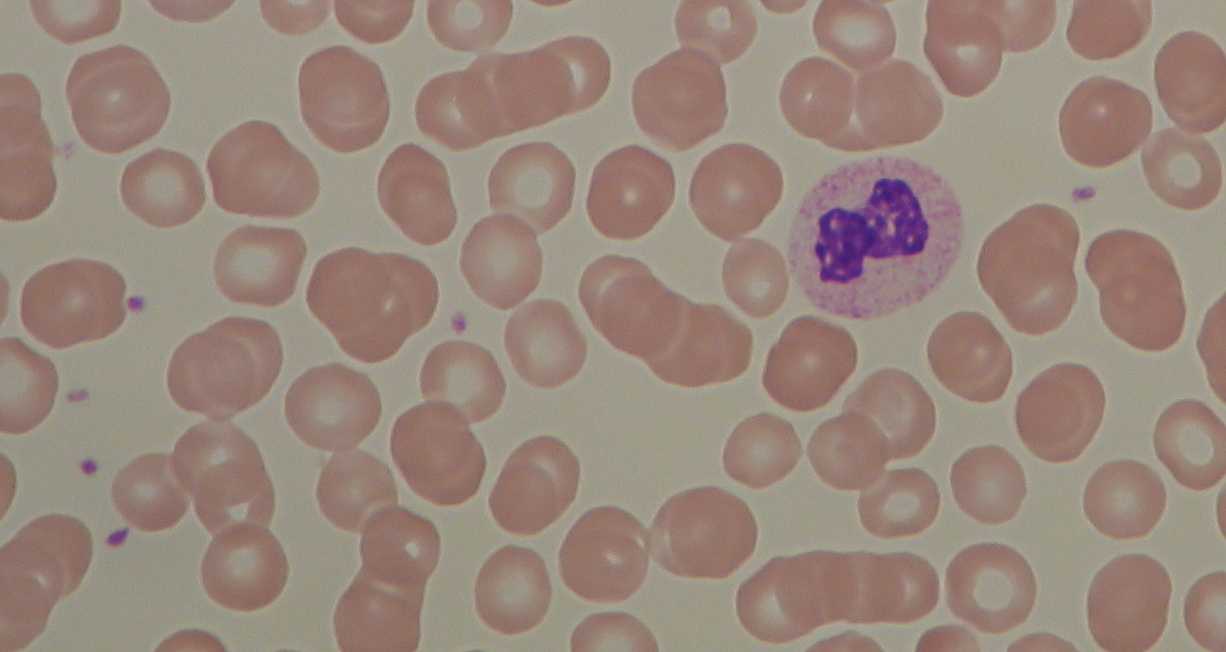
\includegraphics[width = 2.6in]{../images/originalCHT.jpg}}
  \subcaption{Original image}
\end{minipage}%
\begin{minipage}{.5\textwidth}
  \centering
  \fbox{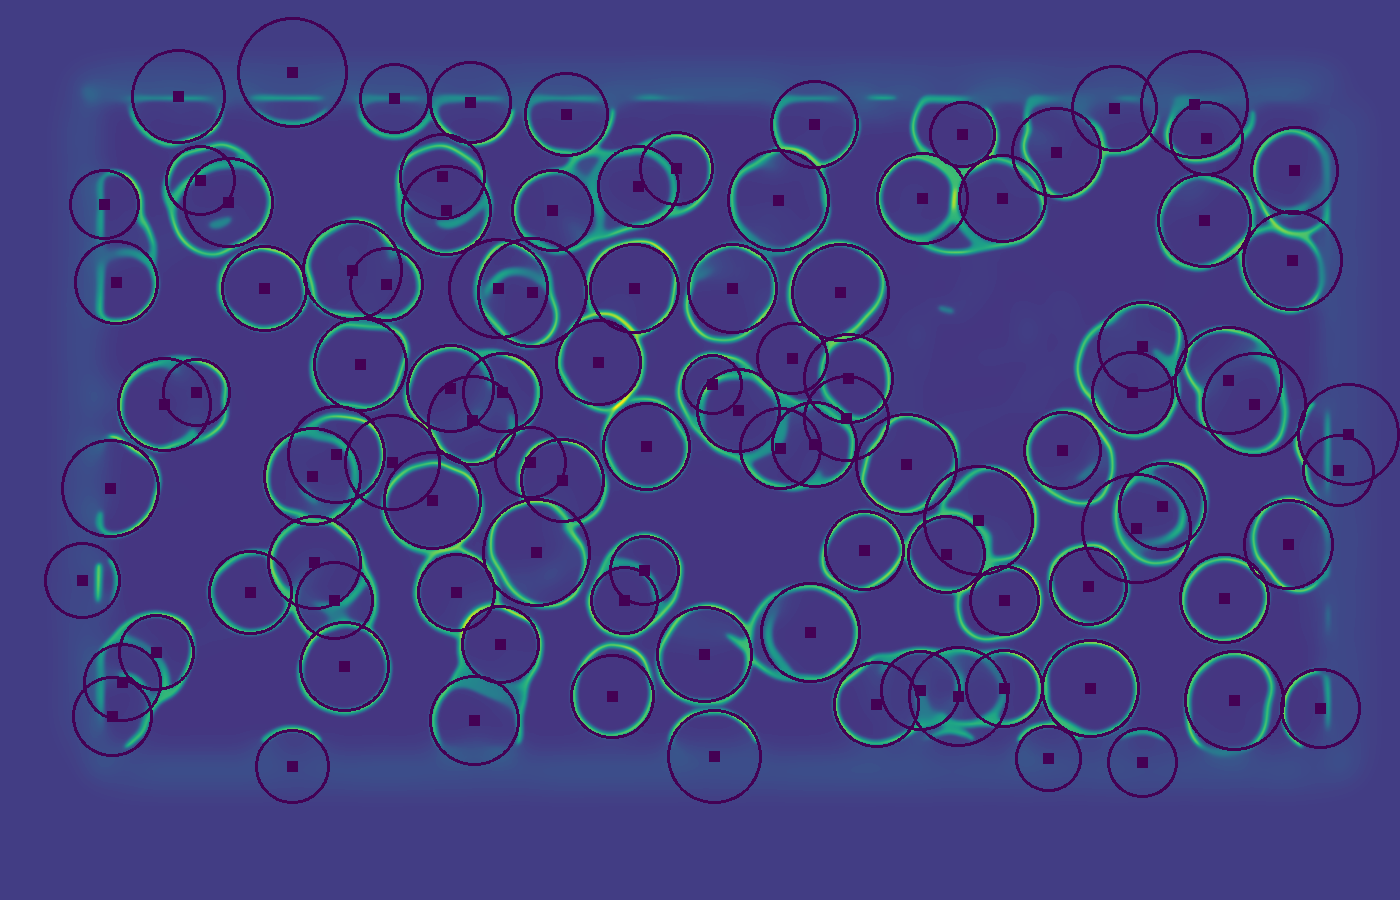
\includegraphics[width = 3.1in]{../images/cht.png}}
  \subcaption{Output CHT image}
\end{minipage}
  \caption{Circle Hough Transform applied to count red blood cells}
  \label{fig:cht_output}
\end{figure}

\begin{figure}[H]
\centering
\begin{minipage}{.5\textwidth}
  \centering
  \fbox{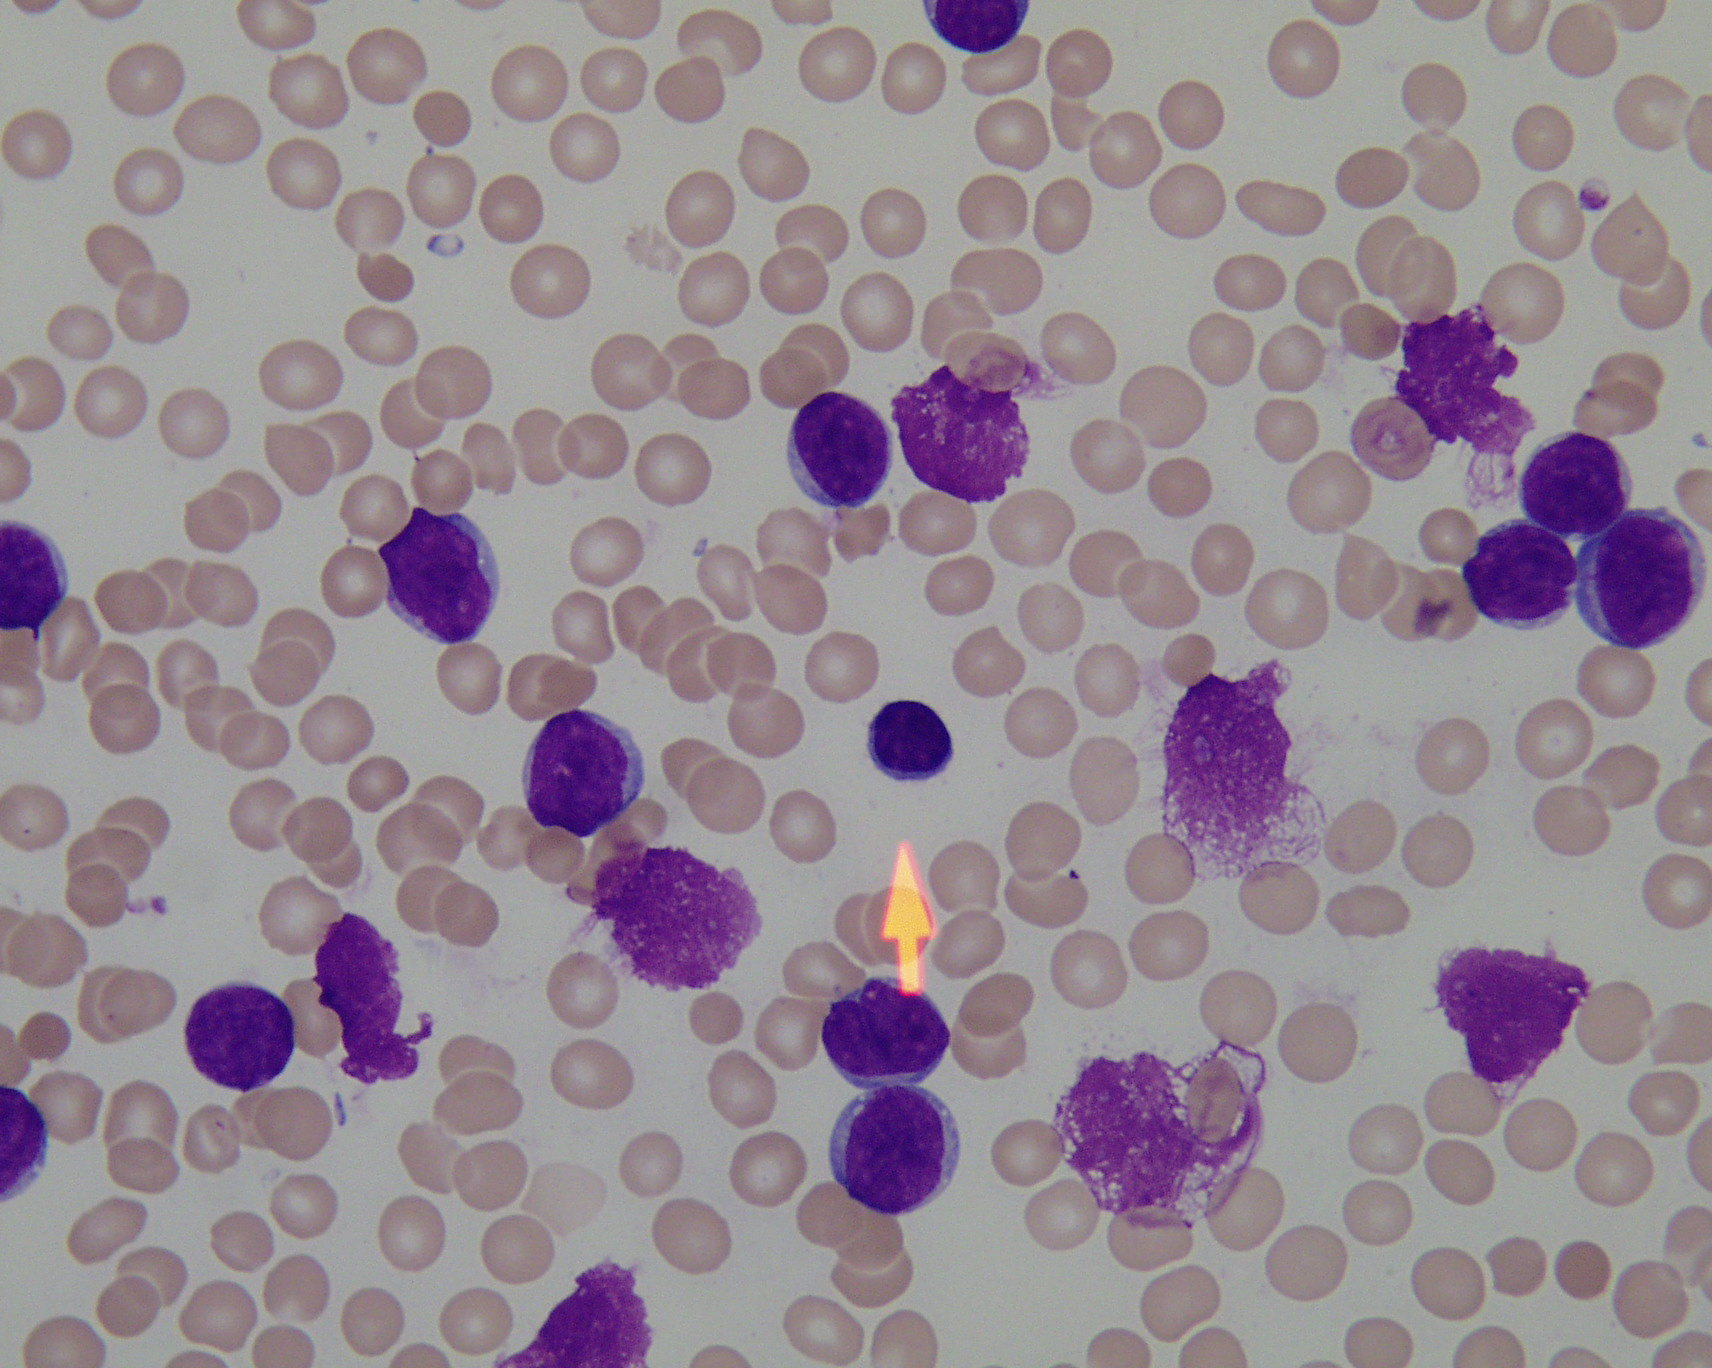
\includegraphics[width = 2.6in]{../images/originalWatershed.jpg}}
  \subcaption{Original image}
\end{minipage}%
\begin{minipage}{.5\textwidth}
  \centering
  \fbox{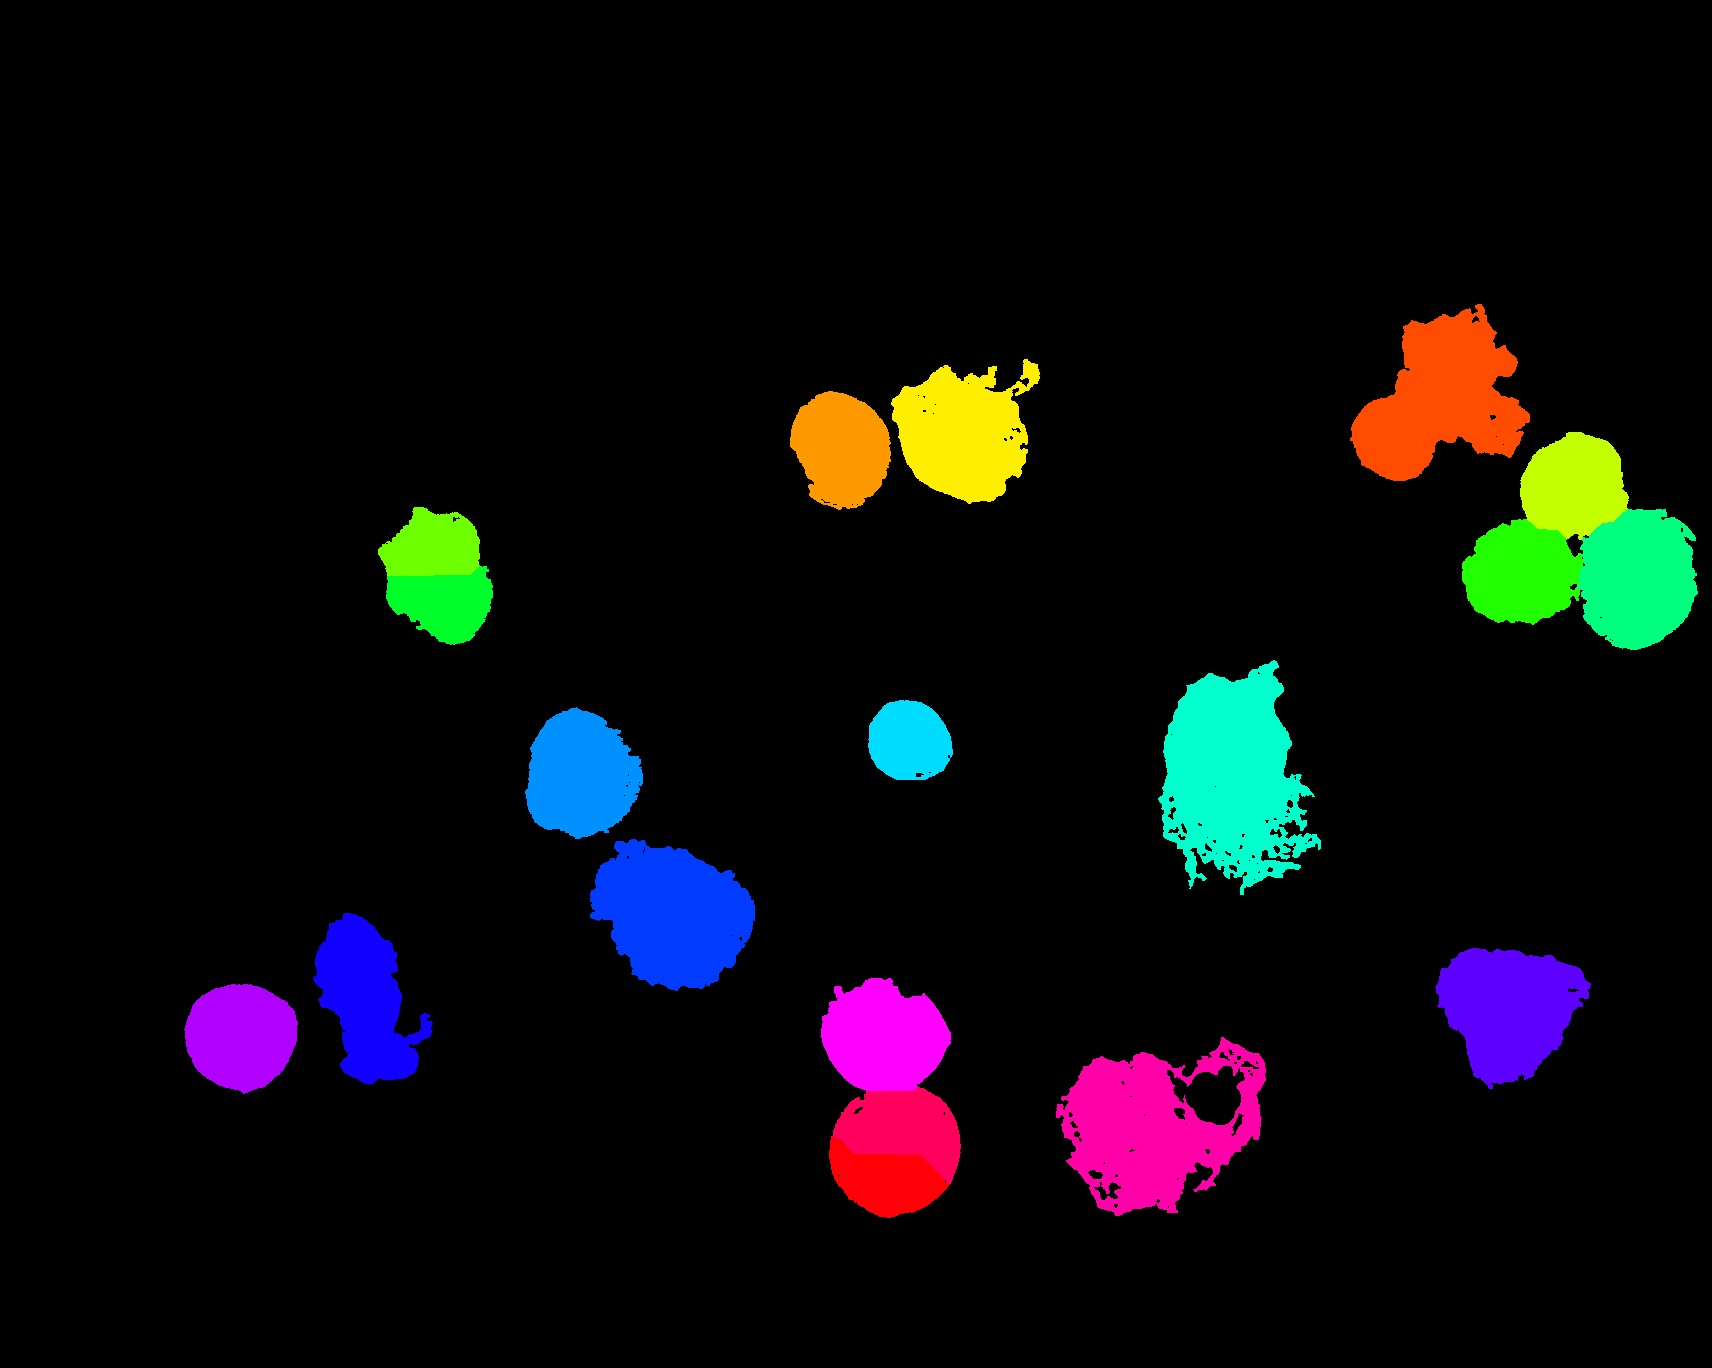
\includegraphics[width = 2.6in]{../images/watershed_color.jpg}}
  \subcaption{Output Watershed image}
\end{minipage}
  \caption{Watershed applied to count white blood cells}
  \label{fig:watershed_output}
\end{figure}

\begin{figure}[H]
\centering
\begin{minipage}{.5\textwidth}
  \centering
  \fbox{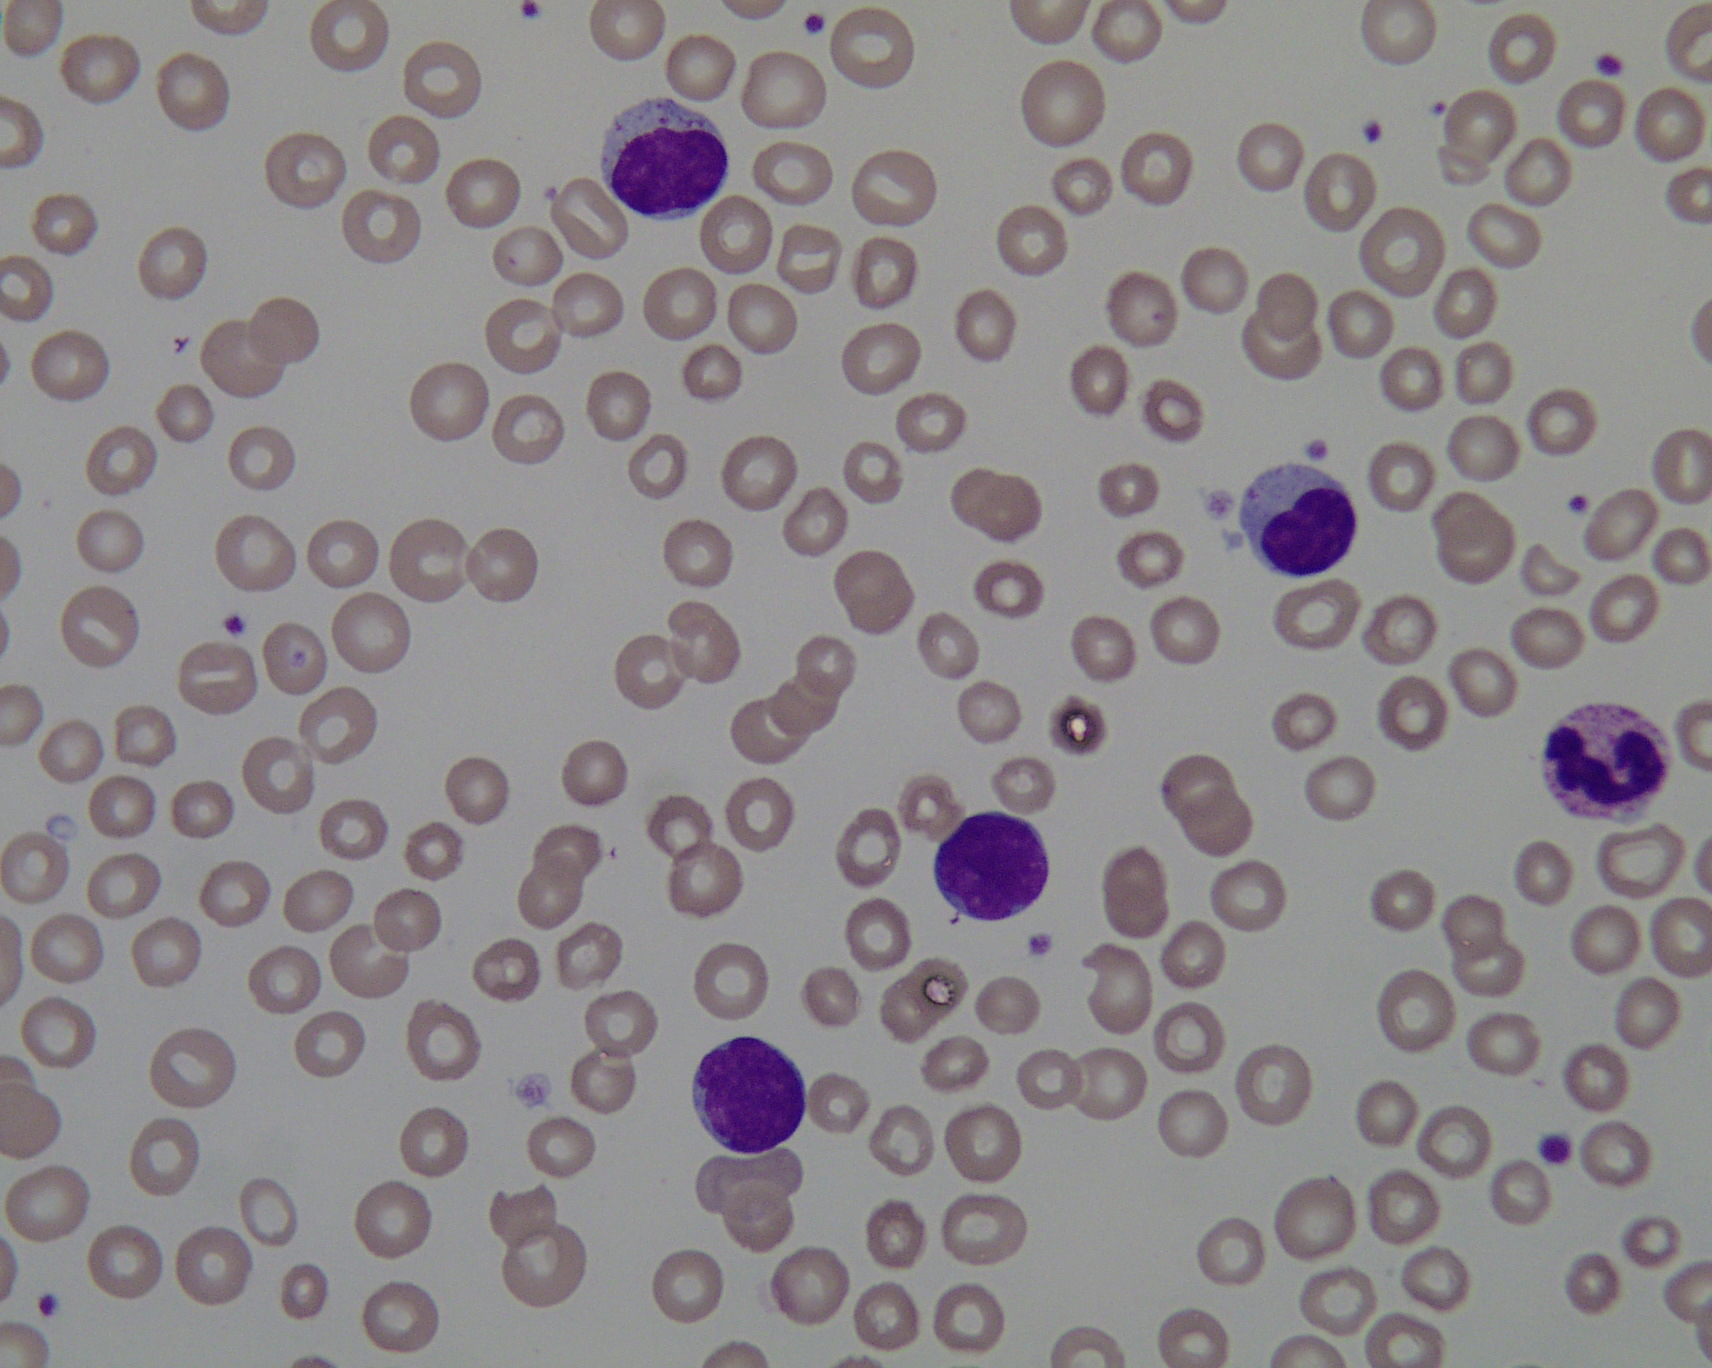
\includegraphics[width = 2.6in]{../images/originalCCL.jpg}}
  \subcaption{Original image}
\end{minipage}%
\begin{minipage}{.5\textwidth}
  \centering
  \fbox{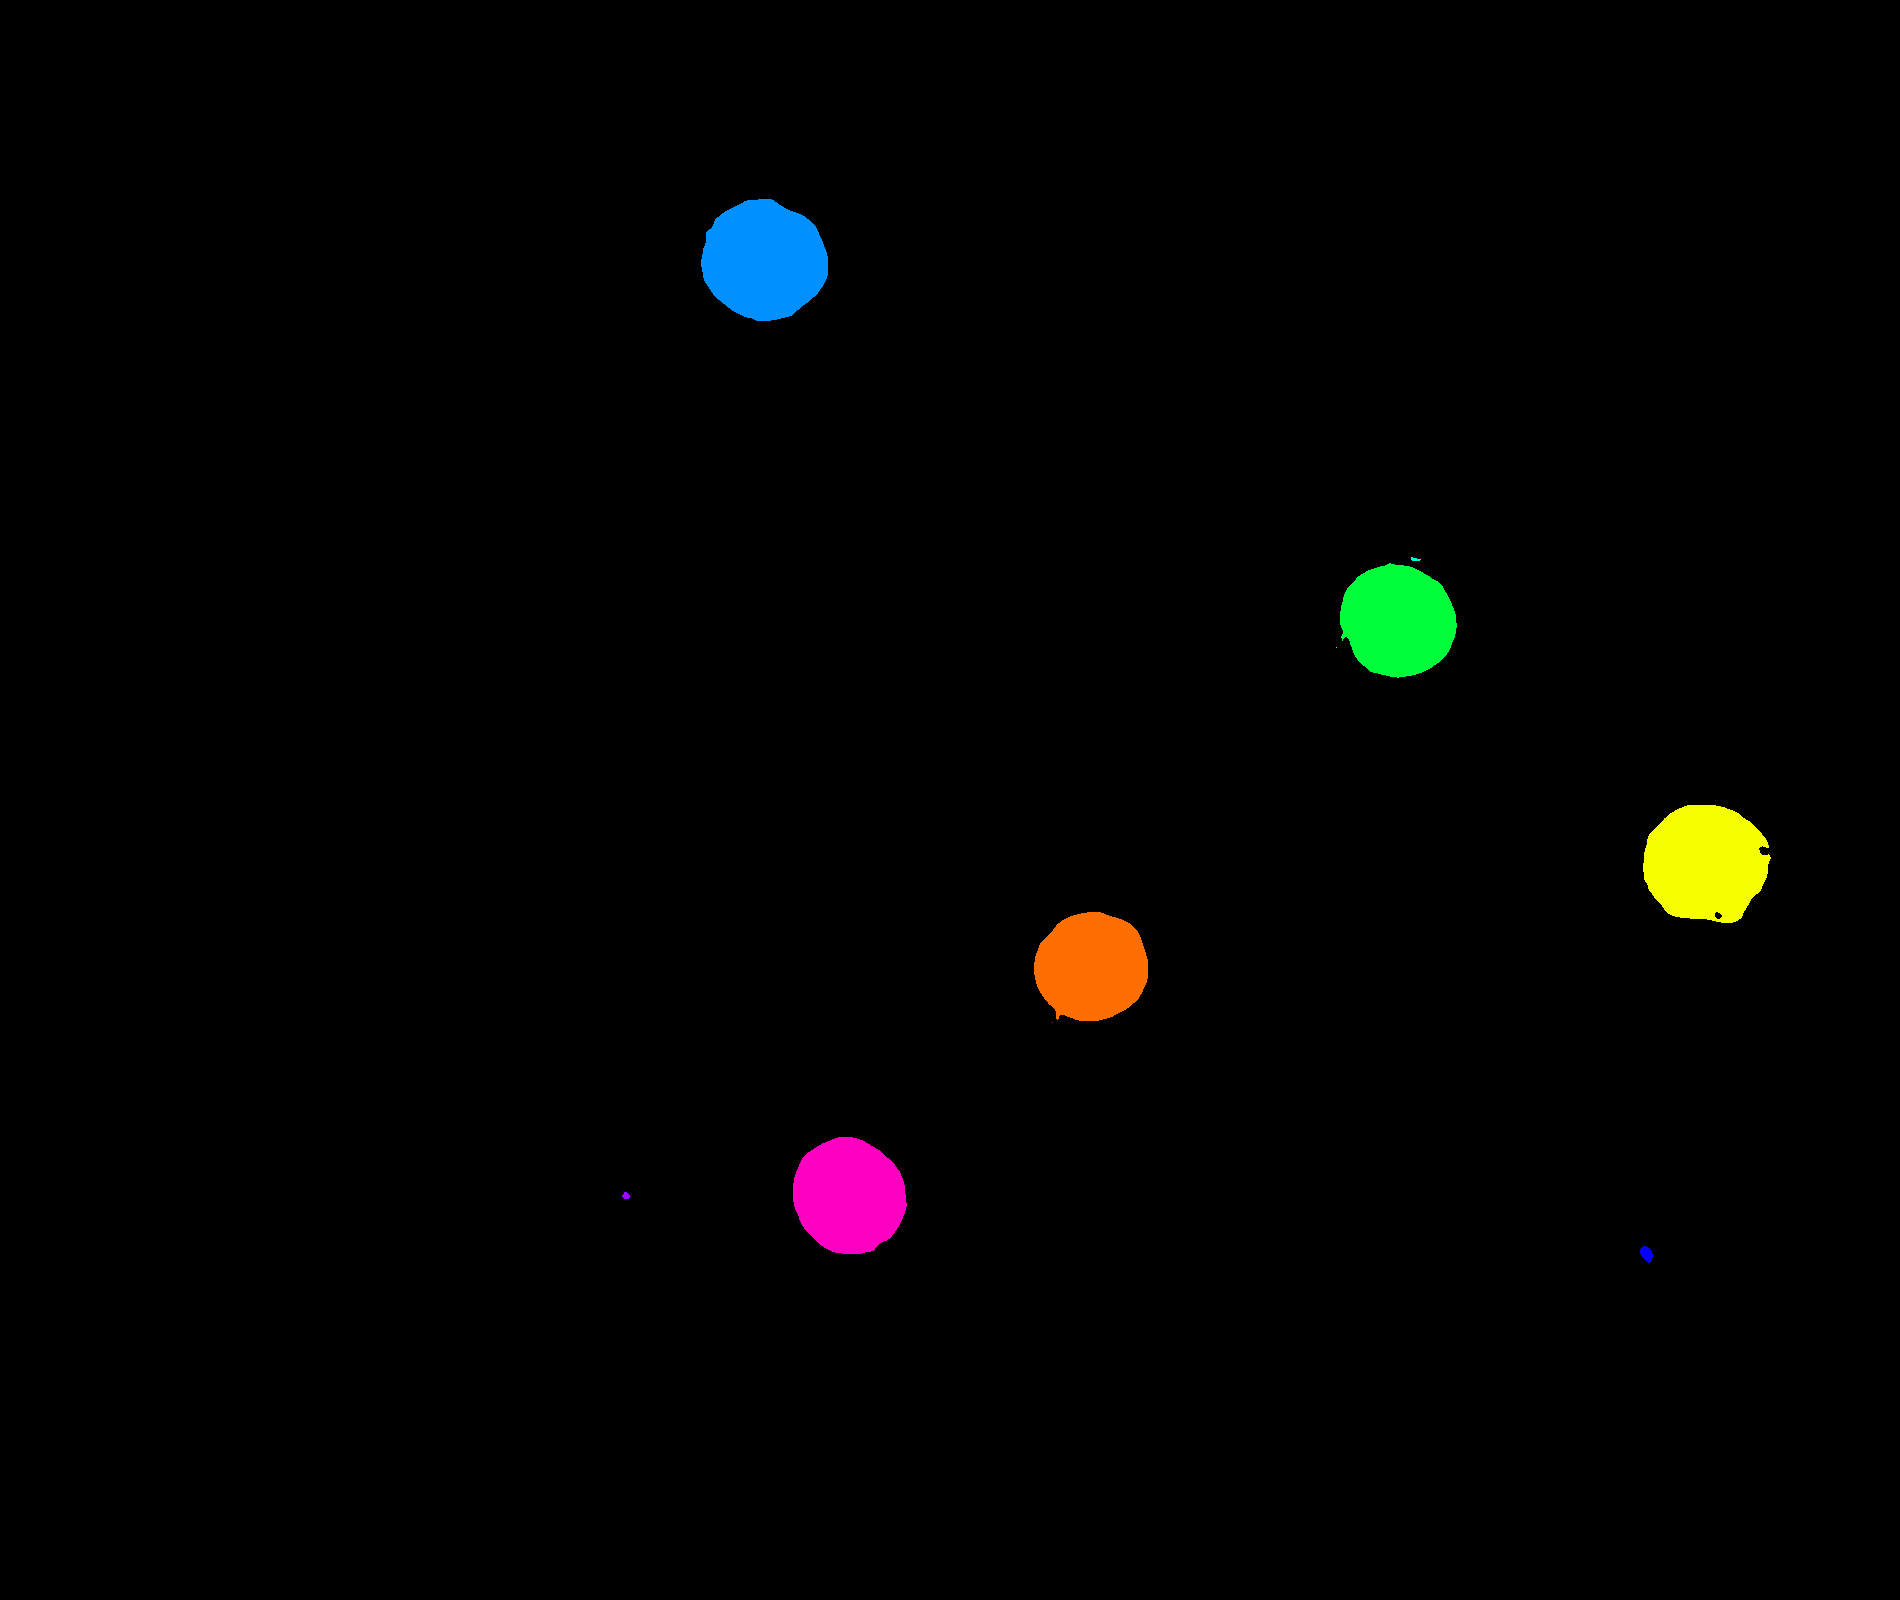
\includegraphics[width = 2.6in]{../images/ccl.png}}
  \subcaption{Output CCL image}
\end{minipage}
  \caption{Connected Component Labeling applied to count white blood cells}
  \label{fig:ccl_output}
\end{figure}

\vspace{-0.1in}

\section{Conclusion}
In conclusion, both models performed very well detecting and counting the blood cells, each one with its advantages and disadvantages.
But the DO-UNet model outperformed SegNet because of the noise generated using SegNet, especially when it comes to platelets since they are very similiar to that noise.

\newpage
